\chapter{Desenvolvimento}
\label{cap:desenvolvimento}

Este capítulo apresenta o desenvolvimento do estudo de caso com Microsserviços e \acrshort{ddd}. Ele descreve as etapas para construção do sistema a partir de requisitos funcionais e não-funcionais.

\section{Ciclo de Vida do Desenvolvimento de Software}
\citeonline{barbaraLiskov} descreve 6 etapas no ciclo de vida de um software: Análise de requisitos, \english{Design}, Implementação e Teste, Teste de aceitação, Produção e Manutenção. A Figura \ref{fig:ciclo-vida} ilustra essas etapas. 

\begin{figure}[H]
    \centering
    \caption{Ciclo de Vida do Desenvolvimento de Software}
    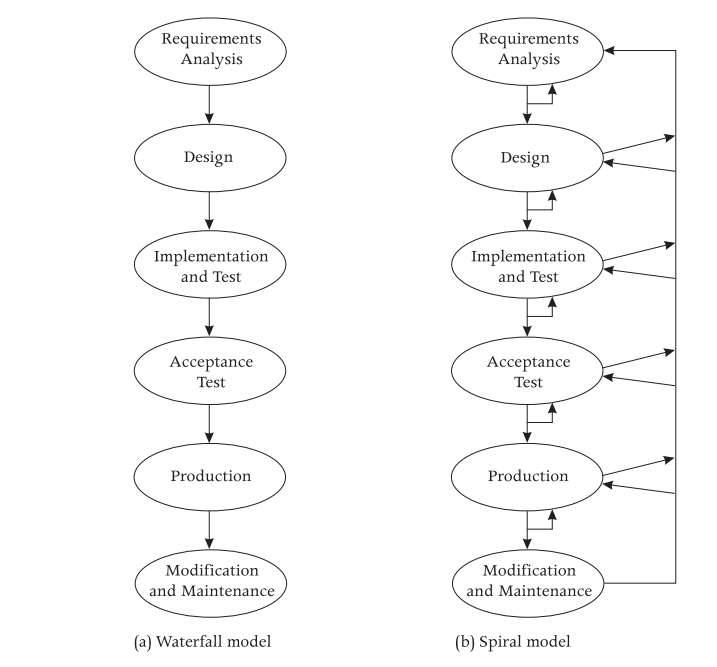
\includegraphics[width=0.8\textwidth]{media/software-life-cycle.png}
    \fonte{\citeonline{barbaraLiskov}}
    \label{fig:ciclo-vida}
\end{figure}

Para este trabalho, os requistos foram definidos no \autoref{cap:metodologia}. Da mesma forma, a fase de manutenção não será abordada, pois o foco é a construção do sistema.

\section{Design}
Esta seção utiliza como entrada os requisitos funcionais e não-funcionais definidos no \autoref{cap:metodologia} para descrever o design do sistema utilizando \acrfull{ams} e \acrfull{ddd}.

Inicialmente, é importante definir os conceitos chaves do sistema, bem como seus relacionamentos. A \autoref{fig:modelo_conceitual} ilustra as abstrações do sistema.

\begin{figure}[H]
    \centering
    \caption{Modelo conceitual do sistema}
    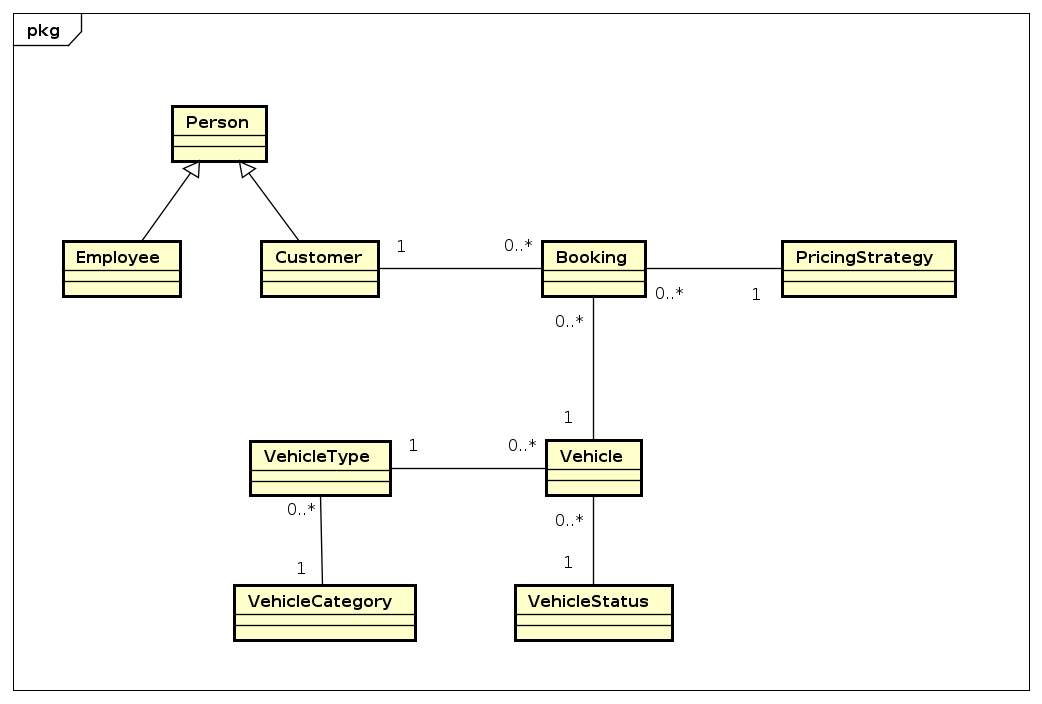
\includegraphics[width=0.8\textwidth]{media/modelo_conceitual.png}
    \fonte{o autor}
    \label{fig:modelo_conceitual}
\end{figure}

O sistema tem como componente principal a entidade \texit{Booking} que está relacionada com um \english{Vehicle} e um \english{Customer}. Cada \english{Vehicle} possui um \english{VehicleType} que tem como função agrupar veículos com características similares. Além disso, cada reserva contém uma \english{PricingStrategy} que é responsável por calcular o preço da reserva baseado em diferentes critérios. Um \english{Customer} é um subtipo de \english{Person}. Da mesma forma, o \english{Employee} é um subtipo de \english{Person}.

No contexto deste caso de uso, as abstrações \english{Booking}, \english{Vehicle}, \english{Customer}, \english{Person} e \english{Employee} possuem identidade e ciclo de vida próprios. Portanto, são entidades. Por outro lado, \english{VehicleType} e \english{PricingStrategy} são \acrfull{vo}, pois não possuem identidade própria e são imutáveis. 

\subsection{Bounded Contexts}
Após ter identificado as entidades e \acrfull{vo}, é necessário definir os \acrfull{bc} do sistema. \citeonline{evans2004ddd} define \acrshort{bc} como um limite lógico dentro do qual um modelo é consistente. Além disso, cada \acrshort{bc} possui um ou mais \english{Aggregates}. Nesse sentido, a \autoref{fig:bounded_contexts} ilustra os \acrshort{bc} do sistema.

\begin{figure}[H]
    \centering
    \caption{Bounded Contexts do sistema}
    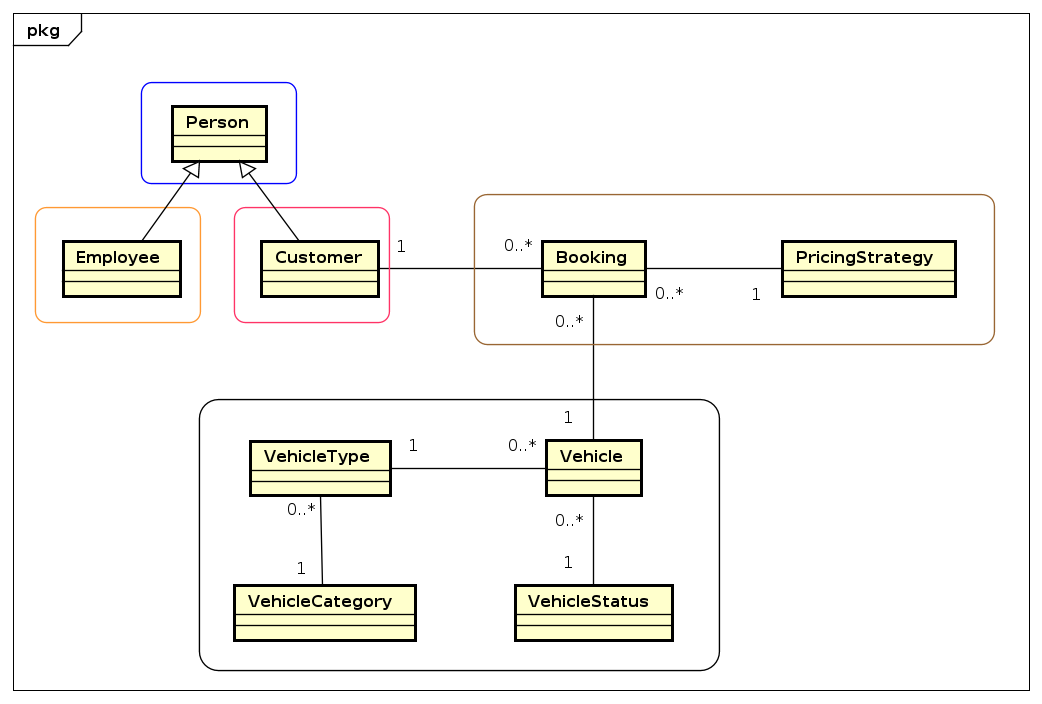
\includegraphics[width=0.8\textwidth]{media/bounded_contexts.png}
    \fonte{o autor}
    \label{fig:bounded_contexts}
\end{figure}

Ao todo, o sistema possui 5 \acrfull{bc}:
\begin{itemize}
    \item \english{Person}: Responsável por gerenciar informações de pessoas e autenticação.
    \item \english{Customer}: Realiza o gerenciamento informações de clientes.
    \item \english{Employee}: Responsável por gerenciar informações de funcionários.
    \item \english{Vehicle}: Está relacionado a estoque de veículos e tipos de veículo.
    \item \english{Booking}: Responsável por gerenciar informações de reservas e estratégias de precificação.
\end{itemize}

\subsection{Microsserviços}
Com os \acrshort{bc} definidos, é possível definir os limites de cada microsserviço. Seguindo as melhores práticas revisadas no \autoref{cap:trabalhos}, cada \acrshort{bc} é mapeado em um microsserviço. A \autoref{fig:microsservicos} ilustra a divisão dos microsserviços.

\begin{figure}[H]
    \centering
    \caption{Microsserviços do sistema}
    \fbox{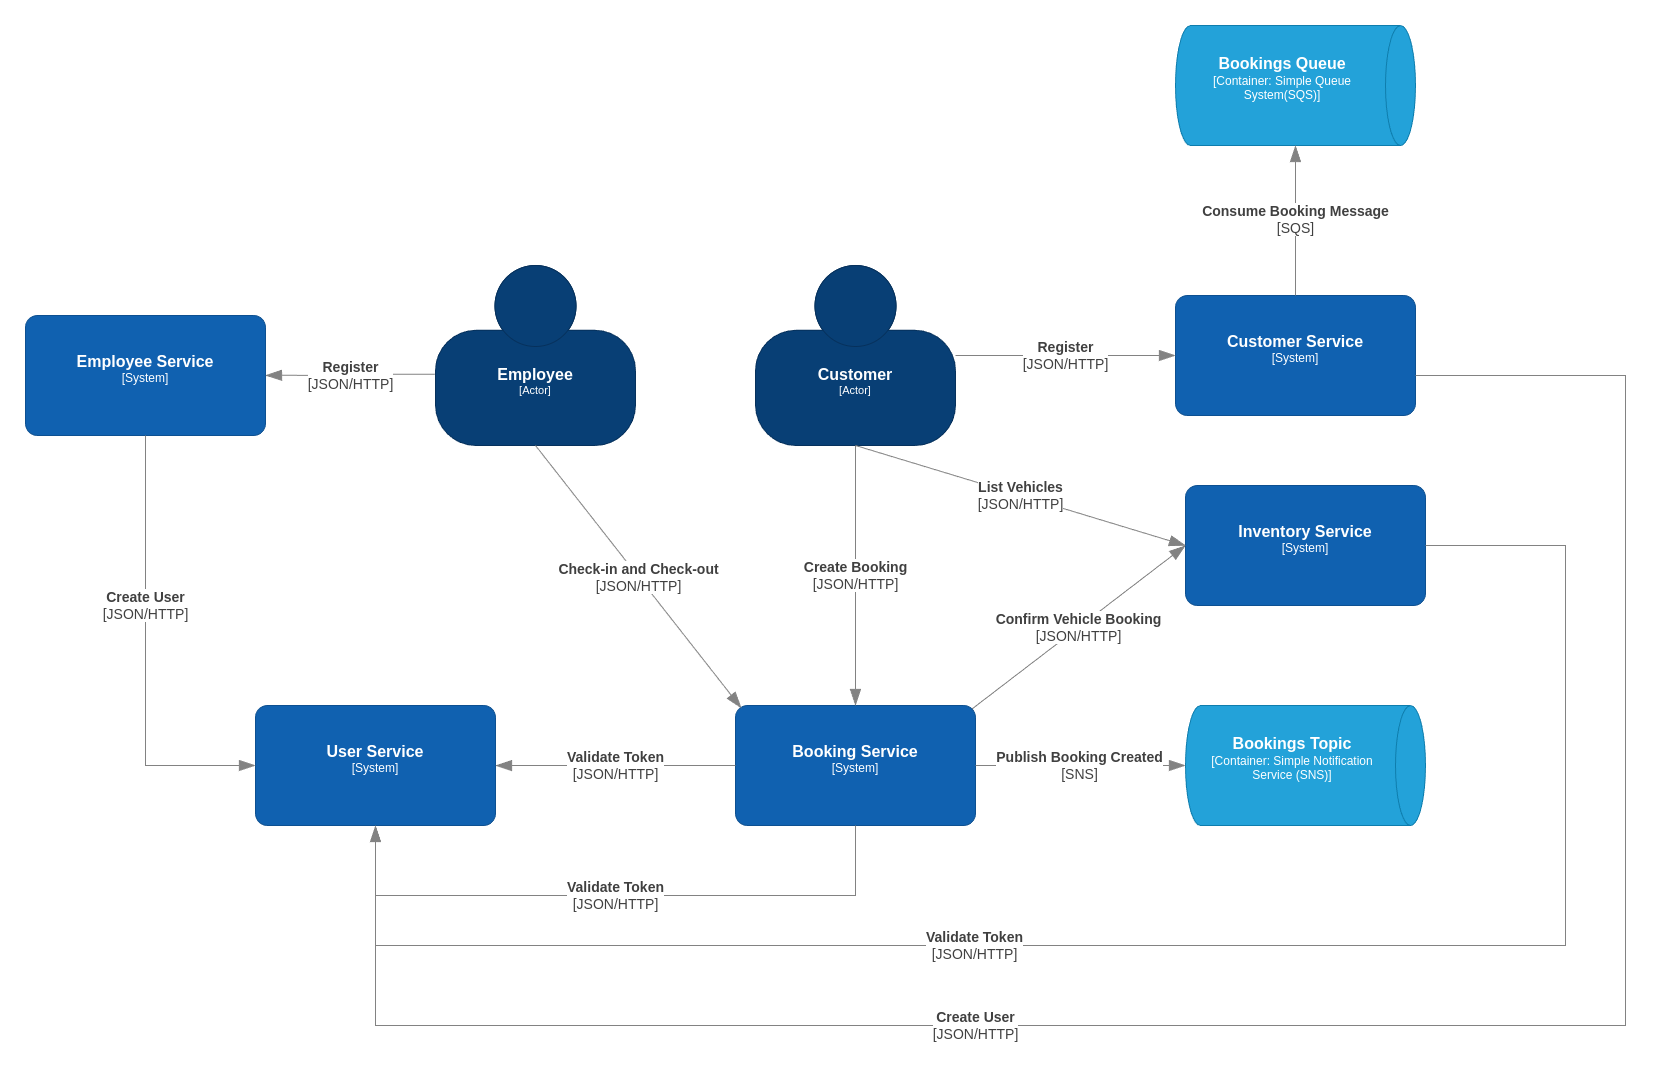
\includegraphics[width=0.8\textwidth]{media/microsservicos.png}}
    \fonte{o autor}
    \label{fig:microsservicos}
\end{figure}

Cada microsserviço é responsável por um \acrshort{bc} e possui sua própria base de dados. O \english{User Service} realiza o cadastro e login de todos usuários do sistema, além de validar \english{tokens} de autenticação. O \english{Customer Service} lida com informações de clientes. Esse serviço também consome uma fila de mensagens de reservas e atualiza um contador de reservas para cada usuário. O \english{Employee Service} gerencia informações de funcionários. O \english{Vehicle Service} trata informações de veículos como quantidade em estoque, marca, modelo, cor e tipo. Por fim, o \english{Booking Service} gerencia informações de reservas e estratégias de precificação.

\subsection{Interações entre Microsserviços}
Como mencionado no \autoref{cap:fundamentacao}, há duas formas principais para estabelecer a comunicação entre microsserviços: síncrona e assíncrona. Para este caso de uso, é utilizada a comunicação assíncrona com a utilização de tópicos e filas de mensagens. A comunicação assíncrona é preferível, pois permite que os microsserviços sejam escalados independentemente, não bloqueia o fluxo de execução e possui maior resiliência. O \english{Booking Service} publica uma mensagem em um tópico de reservas toda vez que uma nova reserva é criada. O \english{Customer Service} consome essa mensagem e atualiza o contador de reservas do usuário.

No entanto, há muitas situações em que a comunicação síncrona é necessária, pois o cliente precisa de uma resposta mediata. Uma opção muito comum é utilizar \english{API Restful} com o protocolo HTTP. Por exemplo, no momento de criação de uma nova reserva o \english{Booking Service} precisa verificar a disponibilidade de veículos no \english{Inventory Service}. Nesse caso, o \english{Booking Service} envia uma requisição HTTP para o \english{Inventory Service} e aguarda a resposta.

\subsection{Principais casos de uso}
A seguir são detalhadas as interações entre os microsserviços para os principais casos de uso do sistema. Especificamente, são descritos os casos de uso que compõem o ciclo de vida de uma reserva ilustrado no \autoref{fig:ciclo-reserva}.

\begin{figure}[H]
    \centering
    \caption{Ciclo de vida de uma reserva}
    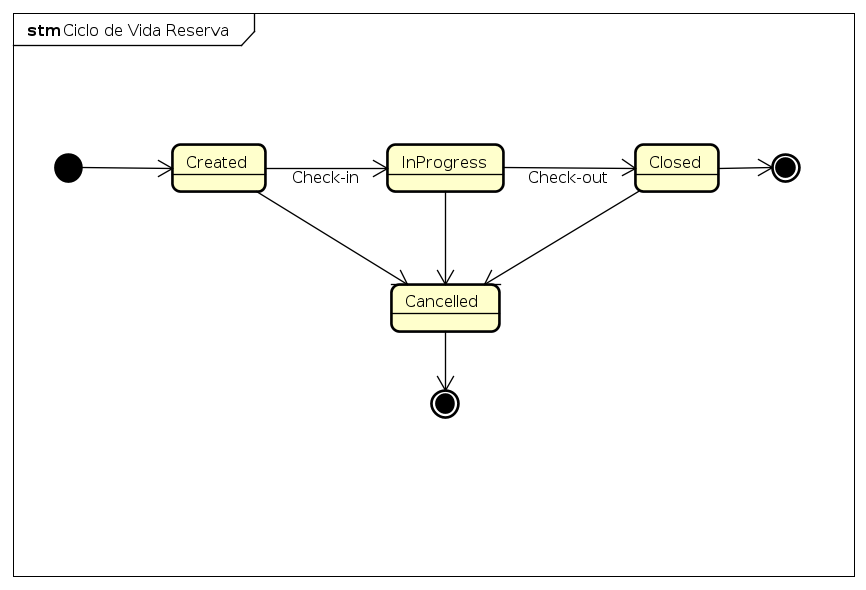
\includegraphics[width=0.8\textwidth]{media/ciclo-reserva.png}
    \fonte{o autor}
    \label{fig:ciclo-reserva}
\end{figure}

\subsubsection{Criar reserva}
A \autoref{fig:realizar-reserva} ilustra o fluxo de criação de uma reserva. Inicialmente, o cliente realiza o login no \english{User Service} e recebe um token como resposta. Em seguida, ele acessa o \english{Vehicle Service} para verificar a disponibilidade de veículos. Esse verifica se o usuário está autenticado realizando uma chamada para o \english{User Service}. Caso o usuário esteja autenticado, o \english{Vehicle Service} retorna a lista de veículos disponíveis. Posteriormente, O cliente seleciona um veículo e realiza a reserva no \english{Booking Service}. Esse serviço envia uma requisição para o \english{Inventory Service} para decrementar a quantidade de veículos disponíveis e confirmar a reserva. Por fim, o \english{Booking Service} retorna a confirmação da reserva.

\begin{figure}[H]
    \centering
    \caption{Criar reserva}
    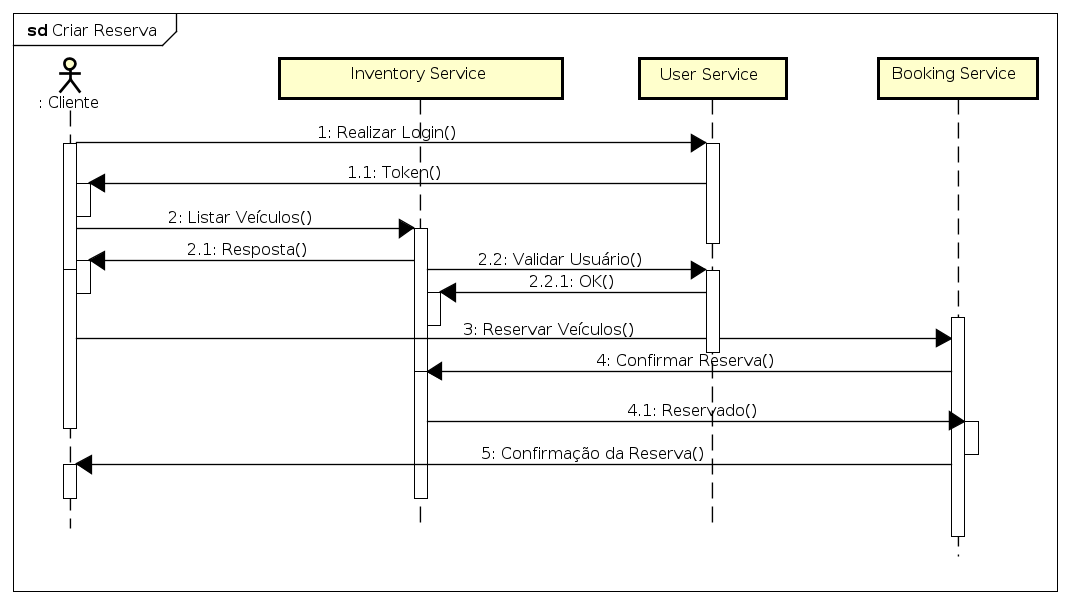
\includegraphics[width=0.8\textwidth]{media/criar-reserva.png}
    \fonte{o autor}
    \label{fig:realizar-reserva}
\end{figure}

\subsubsection{Realizar check-in}
A \autoref{fig:realizar-checkin} ilustra o fluxo de realizar um check-in. Primeiramente, o funcionário realiza o login no \english{User Service} e recebe um token como resposta. Em seguida, ele acessa o \english{Booking Service} para realizar o check-in. Esse serviço verifica se o usuário está autenticado realizando uma chamada para o \english{User Service}. Caso o usuário esteja autenticado, o \english{Booking Service} realiza o check-in e retorna a confirmação.

\begin{figure}[H]
    \centering
    \caption{Realizar check-in}
    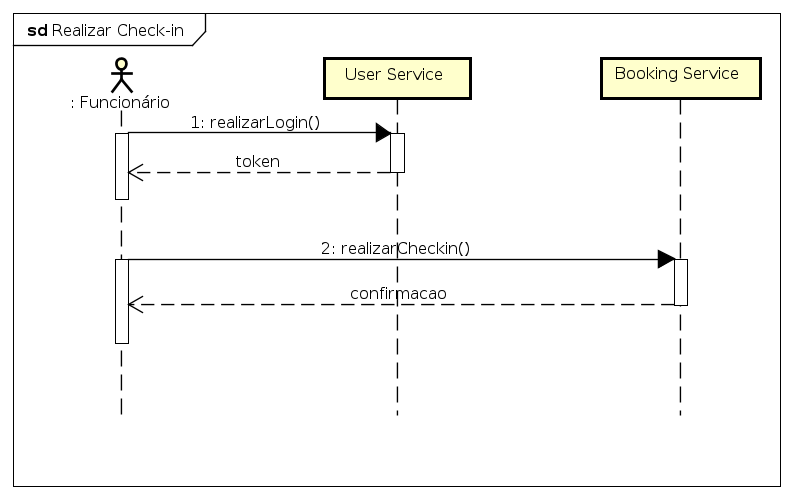
\includegraphics[width=0.8\textwidth]{media/realizar-checkin.png}
    \fonte{o autor}
    \label{fig:realizar-checkin}
\end{figure}

\subsubsection{Realizar check-out}
A \autoref{fig:realizar-checkout} ilustra o fluxo de realizar um check-out. Inicialmente, o funcionário realiza a autenticação no \english{User Service} e recebe um token como resposta. Posteriormente, ele acessa o \english{Booking Service} para realizar o check-out. Esse serviço verifica se o usuário está autenticado realizando uma chamada para o \english{User Service}. Caso o usuário esteja autenticado, o \english{Booking Service} realiza o check-out e retorna a confirmação.

\begin{figure}[H]
    \centering
    \caption{Realizar check-out}
    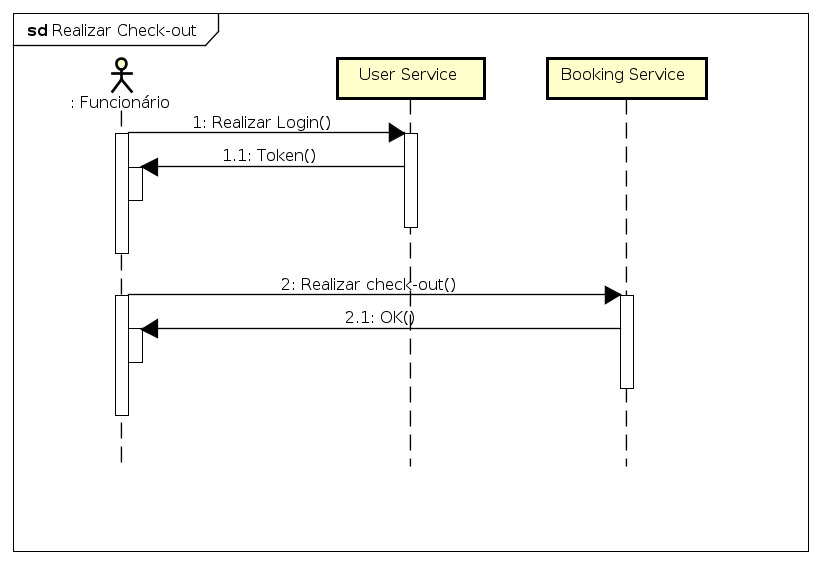
\includegraphics[width=0.8\textwidth]{media/realizar-checkout.png}
    \fonte{o autor}
    \label{fig:realizar-checkout}
\end{figure}

\subsection{User Service}
A \autoref{fig:user-service} apresenta os principais componentes do \english{User Service} na Arquitetura Hexagonal.

\begin{figure}[H]
    \centering
    \caption{User Service}
    \fbox{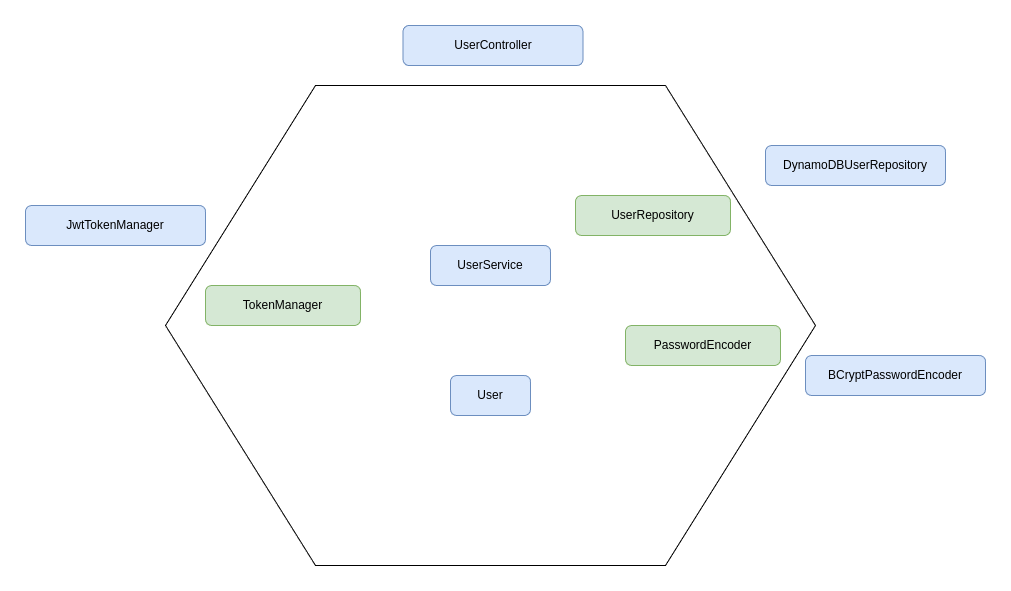
\includegraphics[width=0.8\textwidth]{media/user-service.png}}
    \fonte{o autor}
    \label{fig:user-service}
\end{figure}

Os componentes do \english{Application core} são: \english{User} e \english{UserService}. A aplicação possui as seguintes portas: \english{UserRepository}, \english{PasswordEncoder} e \english{TokenManager}. Por fim, os adaptadores \english{UserController}, \english{DynamoDBUserRepository}, \english{BCryptPasswordEncoder} e \english{JwtTokenManager} são responsáveis por integrar a aplicação com o mundo externo.

\subsection{Customer Service}
A \autoref{fig:customer-service} apresenta os principais componentes do \english{Customer Service} na Arquitetura Hexagonal.

\begin{figure}[H]
    \centering
    \caption{Customer Service}
    \fbox{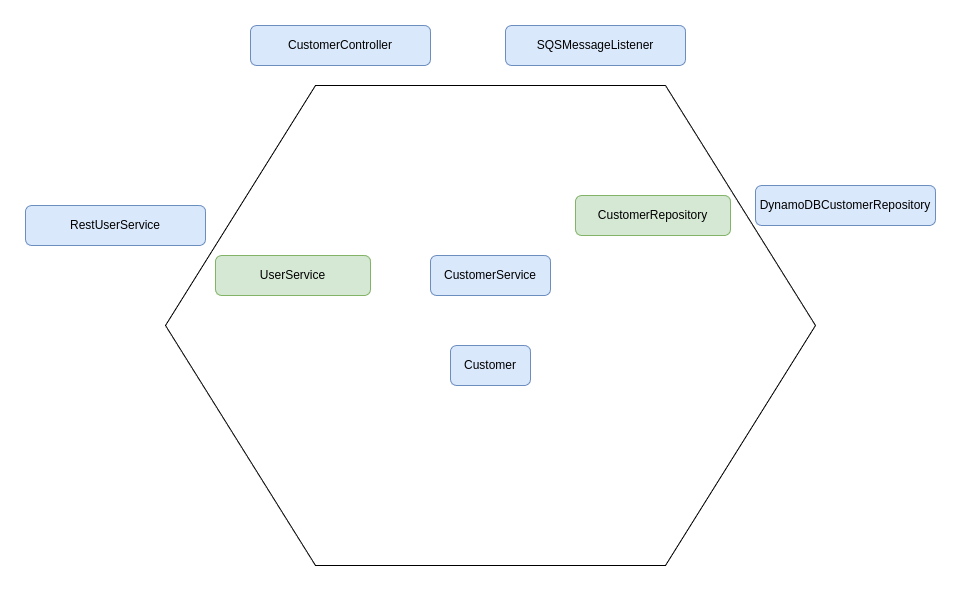
\includegraphics[width=0.8\textwidth]{media/customer-service.png}}
    \fonte{o autor}
    \label{fig:customer-service}
\end{figure}

Nesse serviço, o \english{Application core} é composto por  \english{Customer} e \english{CustomerService}. As portas são: \english{CustomerRepository} e \english{UserService}. Por fim, os adaptadores são: \english{CustomerController}, \english{RestUserService} \english{DynamoDBCustomerRepository} e \english{SQSMessageListener}.

\subsection{Employee Service}
A \autoref{fig:employee-service} apresenta os principais componentes do \english{Employee Service} na Arquitetura Hexagonal.

\begin{figure}[H]
    \centering
    \caption{Employee Service}
    \fbox{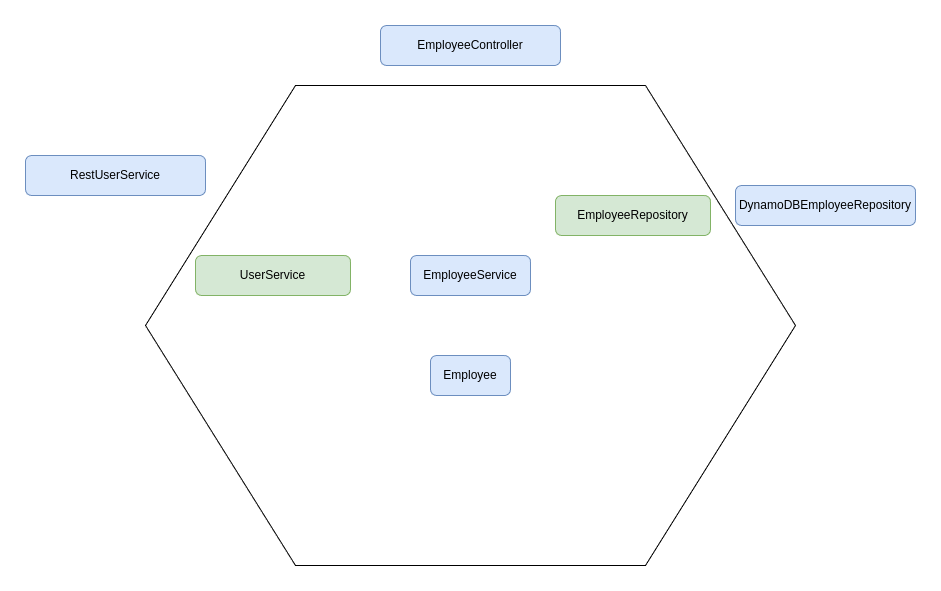
\includegraphics[width=0.8\textwidth]{media/employee-service.png}}
    \fonte{o autor}
    \label{fig:employee-service}
\end{figure}

O \english{Application core} é composto por \english{Employee} e \english{EmployeeService}. As portas são: \english{EmployeeRepository} e \english{UserService}. Por fim, os adaptadores são: \english{EmployeeController}, \english{DynamoDBEmployeeRepository} e \english{RestUserService}.

\subsection{Inventory Service}
Essa seção apresenta os principais componentes do \english{Inventory Service} na Arquitetura Hexagonal, ilustrados na \autoref{fig:inventory-service}.

\begin{figure}[H]
    \centering
    \caption{Inventory Service}
    \fbox{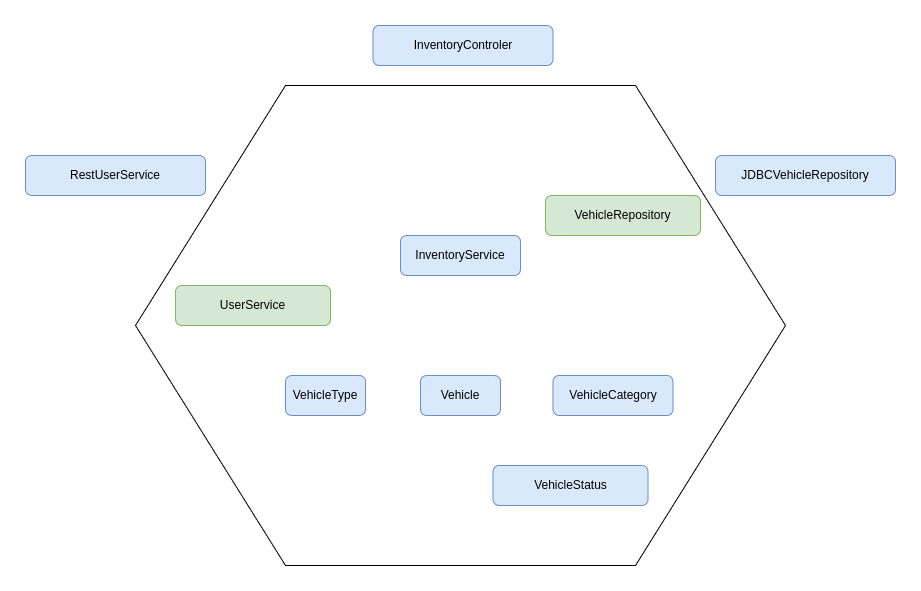
\includegraphics[width=0.8\textwidth]{media/inventory-service.png}}
    \fonte{o autor}
    \label{fig:inventory-service}
\end{figure}

Nessa aplicação, o \english{Application core} é composto por \english{Vehicle}, \english{VehicleType}, \english{VehicleCategory}, \english{VehicleStatus} e \english{InventoryService}. As portas são: \english{VehicleRepository} e \english{UserService}. Por fim, os adaptadores são: \english{InventoryController}, \english{JDBCInventoryRepository} e \english{RestUserService}.

\subsection{Booking Service}
A \autoref{fig:booking-service} apresenta os principais componentes do \english{Booking Service} na Arquitetura Hexagonal.

\begin{figure}[H]
    \centering
    \caption{Booking Service}
    \fbox{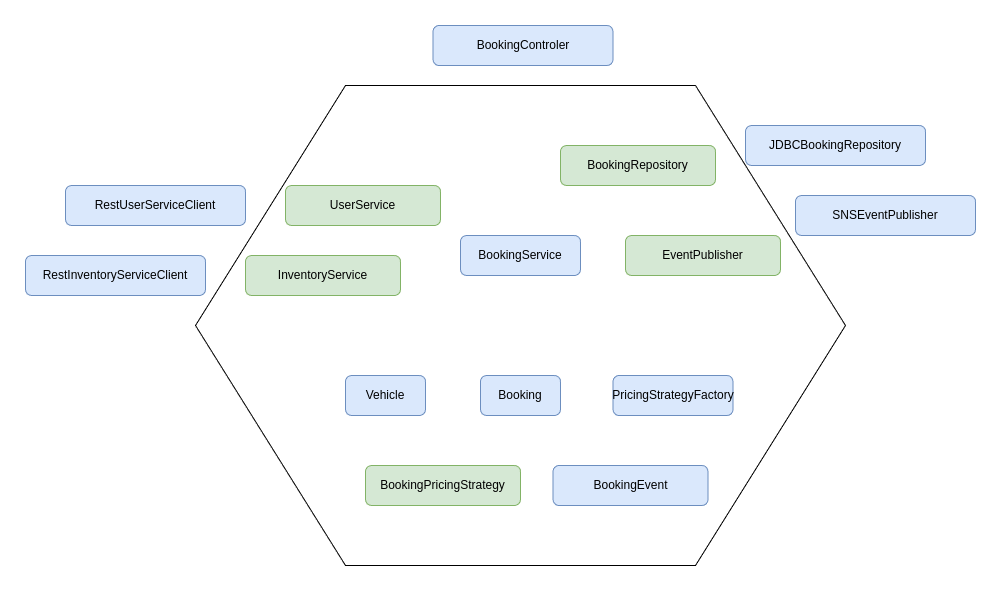
\includegraphics[width=0.8\textwidth]{media/booking-service.png}}
    \fonte{o autor}
    \label{fig:booking-service}
\end{figure}

O \english{Application core} é composto por \english{Booking}, \english{BookingPricingStrategy}, \english{Vehicle}, \english{PricingStrategyFactory}, \english{BookingEvent} e \english{BookingService}. As portas são: \english{BookingRepository}, \english{EventPublisher}, \english{UserService} e \english{InventoryService}. Por fim, os adaptadores são: \english{BookingController}, \english{JDBCBookingRepository}, \english{SNSEventPublisher}, \english{RestUserServiceClient} e \english{RestInventoryServiceClient}.

\section{Implementação}
Esta seção apresenta os trechos de código chaves para a implementação do caso de uso. O código completo pode ser encontrado no repositório do projeto \footnote{\url{https://github.com/C0lliNN/CarroFacil}}.

\subsection{Login de usuário}
O \autoref{cod:login} apresenta o método para realizar login de um usuário. Esse método recebe um \english{LoginRequest} contendo o email e senha do usuário. Em seguida, ele busca o usuário no repositório e compara a senha informada com a senha armazenada no banco de dados. Caso a senha seja válida, o método retorna um \english{UserResponse} contendo o token de autenticação. O procedimento lança exceções caso o email não seja encontrado ou a senha seja inválida.

\begin{codigo}[H]
    \begin{lstlisting}[language=Java]
public class UserService {
    private final UserRepository repository;
    private final PasswordEncoder passwordEncoder;
    private final TokenManager tokenManager;

    public UserResponse login(LoginRequest request) {
        User user = repository.findByEmail(request.email()).
                orElseThrow(() -> new EmailNotFoundException("The email '%s' could not be found.", request.email()));

        if (!passwordEncoder.comparePasswordAndHash(request.password(), user.getPassword())) {
            throw new IncorrectPasswordException("The provided password is incorrect.");
        }

        return createUserResponseWithToken(user);
    }

    // Other methods
}
    \end{lstlisting}
    \caption{Método para realizar login}
    \label{cod:login}
\end{codigo}

\subsection{Cadastro de Cliente}
O \autoref{cod:cadastro-cliente} apresenta o método para realizar o cadastro de um cliente. Esse método recebe um \english{RegisterRequest} contendo o nome, email e senha do cliente. Em seguida, ele realiza o cadastro do usuário no \english{User Service} e cria um cliente no \english{Customer Service}. Por fim, o método retorna um \english{CustomerResponse} contendo as informações do cliente.

\begin{codigo}[H]
    \begin{lstlisting}[language=Java]
public class CustomerService {
    private final UserServiceClient userServiceClient;
    private final CustomerRepository customerRepository;

    public CustomerResponse register(RegisterRequest request) {
        User user = userServiceClient.register(request.name(), request.email(), request.password());

        Customer customer = Customer.builder()
                .name(request.name())
                .userId(user.getId())
                .build();

        return CustomerResponse.fromCustomer(customerRepository.save(customer), user);
    }

// Other methods
    }
    \end{lstlisting}
    \caption{Método para realizar cadastro de cliente}
    \label{cod:cadastro-cliente}
\end{codigo}

\subsection{Realizar Reserva}
O \autoref{cod:realizar-reserva} apresenta o método para realizar uma reserva. Esse método recebe um \english{BookingRequest} contendo as informações da reserva. Em seguida, ele busca o veículo no \english{Inventory Service} e realiza a reserva no \english{Booking Service}. Além disso, o método publica um evento que poderá ser consumido por outros serviços. Por fim, o método retorna um \english{BookingResponse} contendo as informações da reserva.

\begin{codigo}[H]
    \begin{lstlisting}[language=Java]
public class BookingService {
    private BookingRepository bookingRepository;
    private InventoryClient inventoryClient;
    private BookingEventPublisher bookingEventPublisher;

    public BookingResponse createBooking(BookingRequest bookingRequest) {
        Booking booking = bookingRequest.createBooking();
        Vehicle vehicle = inventoryClient.getVehicle(booking.getVehicleId());
        booking.setVehicle(vehicle);

        booking = bookingRepository.save(booking);

        bookingEventPublisher.publishBookingEvent(
                new BookingEvent(booking.getId(), booking.getUserId(), vehicle.getId())
        );

        return BookingResponse.from(booking);
    }

    // Other methods
}
    \end{lstlisting}
    \caption{Método para criar reserva}
    \label{cod:realizar-reserva}
\end{codigo}

\subsection{Realizar Check-in}
O \autoref{cod:realizar-check-in} contém o código necessário para realizar um check-in. No \english{BookingService} é possível ver o método \english{checkin} que recebe o id da reserva e realiza o check-in. Esse método busca a reserva no repositório, realiza o check-in e salva a reserva. Toda a operação é executada em uma transação ACID com nível de isolamento de serialização para previnir checkins duplicados. O método \english{checkIn} da classe \english{Booking} é responsável por validar o estado da reserva, atualizar o status e a data de check-in.

\begin{codigo}[H]
    \begin{lstlisting}[language=Java]
public class BookingService {
    private BookingRepository bookingRepository;
    private InventoryClient inventoryClient;
    private BookingEventPublisher bookingEventPublisher;

    @Transactional(isolation = Isolation.SERIALIZABLE)
    public void checkin(int bookingId) {
        Booking booking = bookingRepository.findById(bookingId)
                .orElseThrow(() -> new EntityNotFoundException("Booking not found"));

        booking.checkIn();
        bookingRepository.save(booking);
    }

    // Other methods
}

public class Booking {
    // other fields and methods

    public void checkIn() {
        if (status != Status.CREATED) {
            throw new InvalidBookingStateException("Booking is not in CREATED state");
        }

        status = Status.IN_PROGRESS;
        checkedInAt = LocalDateTime.now();
    }
}
    \end{lstlisting}
    \caption{Métodos para realizar check-in}
    \label{cod:realizar-check-in}
\end{codigo}

\subsection{Realizar Check-out}
O \autoref{cod:realizar-check-out} contém o código necessário para realizar um check-out. No \english{BookingService} é possível ver o método \english{checkout} que recebe o id da reserva e realiza o check-out. Esse método busca a reserva no repositório, realiza o check-out e salva a reserva. Toda a operação é executada em uma transação ACID com nível de isolamento de serialização para previnir checkouts duplicados. O método \english{checkOut} da classe \english{Booking} é responsável por validar o estado da reserva, atualizar o status e a data de check-out.

\begin{codigo}[H]
    \begin{lstlisting}[language=Java]
public class BookingService {
    private BookingRepository bookingRepository;
    private InventoryClient inventoryClient;
    private BookingEventPublisher bookingEventPublisher;

    @Transactional(isolation = Isolation.SERIALIZABLE)
    public void checkout(int bookingId) {
        Booking booking = bookingRepository.findById(bookingId)
                .orElseThrow(() -> new EntityNotFoundException("Booking not found"));

        booking.checkOut();
        bookingRepository.save(booking);
    }

    // Other methods
}

public class Booking {
    // other fields and methods

    public void checkOut() {
        if (status != Status.IN_PROGRESS) {
            throw new InvalidBookingStateException("Booking is not in IN_PROGRESS state");
        }

        status = Status.CLOSED;
        checkedOutAt = LocalDateTime.now();
    }
}
    \end{lstlisting}
    \caption{Métodos para realizar check-out}
    \label{cod:realizar-check-out}
\end{codigo}

\subsection{Comunicação síncrona entre Microsserviços}
O \autoref{cod:rest-inventory-client} demonstra como a comunicação síncrona entre microsserviços é realizada. O método \english{getVehicle} da classe \english{RestInventoryClient} é responsável por obter um veículo do \english{Inventory Service}. Esse método utiliza o \english{RestTemplate} para realizar uma requisição \acrshort{http} para \english{Inventory Service}. É importante notar que a classe \english{RestInventoryClient} implementa a interface de domínio \english{InventoryClient}. Dessa forma o dominio não está acoplado ao mecanismo de comunicação.

\begin{codigo}[H]
    \begin{lstlisting}[language=Java]
public class RestInventoryClient implements InventoryClient {
    private RestTemplate restTemplate;
    private String baseUrl;

    @Override
    public Vehicle getVehicle(int id) {
        HttpHeaders headers = new HttpHeaders();
        headers.set("Authorization", "Bearer " + getToken());
        HttpEntity<VehicleResponse> entity = new HttpEntity<>(headers);

        ResponseEntity<VehicleResponse> response = restTemplate.exchange(baseUrl + "/vehicles/{id}", HttpMethod.GET, entity, VehicleResponse.class, id);
        if (response.getStatusCode().value() == 404) {
            throw new EntityNotFoundException("Vehicle not found");
        }

        if (response.getStatusCode().isError()) {
            throw new RuntimeException("Error while fetching vehicle");
        }

        return response.getBody().toVehicle();
    }
}
    \end{lstlisting}
    \caption{Método para obter um veículo do \english{Inventory Service}}
    \label{cod:rest-inventory-client}
\end{codigo}

\subsection{Comunicação assíncrona entre Microsserviços}
O \autoref{cod:comunicacao-assincrona} apresenta como a comunicação assíncrona entre microsserviços é realizada. A classe \english{SNSEventPublisher} é responsável por publicar eventos de reserva no \english{Booking Service}. O método \english{publishBookingEvent} recebe um evento de reserva, serializa o evento e publica no tópico \acrshort{sns}. Por outro lado, a classe \english{SQSListener} é responsável por ouvir eventos de reserva no \english{Customer Service}. O método \english{listen} recebe uma mensagem do \acrshort{sqs}, desserializa a mensagem e incrementa o contador de reservas do usuário. Da mesma forma que na comunicação síncrona, o domínio não está acoplado ao mecanismo de comunicação.

\begin{codigo}[H]
    \begin{lstlisting}[language=Java]
// class in Booking Service
public class SNSEventPublisher implements BookingEventPublisher {
    private final SnsClient snsClient;
    private final ObjectMapper objectMapper;

    private String topicArn;

    public void publishBookingEvent(BookingEvent bookingEvent) {
        String message = objectMapper.writeValueAsString(bookingEvent);

        PublishRequest request = PublishRequest.builder()
                .topicArn(topicArn)
                .message(message)
                .build();

        PublishResponse response = snsClient.publish(request);
    }
}

// class in Customer service
public class SQSListener {
    private final CustomerService service;
    private final ObjectMapper objectMapper;

    @SqsListener(queueNames = "${aws.queues.bookings}")
    public void listen(Message message) {
        try {
            MessageBody body = objectMapper.readValue(message.body(), MessageBody.class);
            BookingMessage bookingMessage = objectMapper.readValue(body.getMessage(), BookingMessage.class);

            log.info("Received message: {}", bookingMessage);

            service.incrementBookingsCount(bookingMessage.getUserId());
        } catch (Exception e) {
            throw new RuntimeException("Error while processing message", e);
        }
    }
}

    \end{lstlisting}
    \caption{Código para realizar comunicação assíncrona entre microsserviços}
    \label{cod:comunicacao-assincrona}
\end{codigo}

\section{Testes}
Esta seção apresenta os testes realizados para validar os requisitos funcionais e não funcionais do sistema.

\subsection{Testes Unitários}
Os testes unitários foram realizados utilizando o \english{framework} JUnit. O \autoref{cod:unitario-simples} apresenta um teste unitário simples para o método \english{checkIn} da classe \english{Booking}. Esse teste verifica se o status da reserva é alterado para \english{IN\_PROGRESS} e se a data de check-in é definida quando o status é \english{CREATED}. Além disso, o teste verifica se uma exceção é lançada quando o status não é \english{CREATED}.

\begin{codigo}[H]
    \begin{lstlisting}[language=Java]
@Nested
@DisplayName("checkIn method")
class CheckInMethod {

    @Test
    @DisplayName("should change status to IN_PROGRESS and set checkedInAt to current time when status is CREATED")
    void shouldChangeStatusToInProgressAndSetCheckedInAtToCurrentTimeWhenStatusIsCreated() {
        Booking booking = new Booking();
        booking.setStatus(Booking.Status.CREATED);

        booking.checkIn();

        assertEquals(Booking.Status.IN_PROGRESS, booking.getStatus());
        assertNotNull(booking.getCheckedInAt());
    }

    @Test
    @DisplayName("should throw InvalidBookingStateException when status is not CREATED")
    void shouldThrowInvalidBookingStateExceptionWhenStatusIsNotCreated() {
        Booking booking = new Booking();
        booking.setStatus(Booking.Status.CANCELLED);

        assertThrows(InvalidBookingStateException.class, booking::checkIn);
    }
}
    \end{lstlisting}
    \caption{Teste unitário simples}
    \label{cod:unitario-simples}
\end{codigo}

\subsection{Testes de Integração}
O framework Mockito é utilizado para execucação dos testes de integração de maneira isolada. O \autoref{cod:test-integracao} apresenta um teste de integração para o método \english{checkin} da classe \english{BookingService}. Esse teste verifica se uma exceção é lançada quando a reserva não é encontrada e se o status da reserva é alterado para \english{IN\_PROGRESS} quando a reserva é encontrada. Além disso, o teste verifica se o método \english{save} do repositório é chamado uma vez.

\begin{codigo}[H]
    \begin{lstlisting}[language=Java]
@Nested
@DisplayName("method: checkin")
class Checkin {

    @Mock
    private BookingRepository bookingRepository;

    @Test
    @DisplayName("when booking is not found, then it should throw a EntityNotFoundException")
    void whenBookingIsNotFound_thenItShouldThrowAEntityNotFoundException() {
        assertThrows(EntityNotFoundException.class, () -> bookingService.checkin(1));
    }

    @Test
    @DisplayName("when all operations are successful, then it should checkin the booking")
    void whenAllOperationsAreSuccessful_thenItShouldCheckinTheBooking() {
        when(bookingRepository.findById(1)).thenReturn(Optional.of(booking));
        when(bookingRepository.save(booking)).thenReturn(booking);

        bookingService.checkin(1);

        assertEquals(Booking.Status.IN_PROGRESS, booking.getStatus());
        verify(bookingRepository, times(1)).save(booking);
    }
}
    \end{lstlisting}
    \caption{Teste de integração}
    \label{cod:test-integracao}
\end{codigo}

\subsection{Testes de Sistema}
Os testes de sistema são realizados com auxílio do Testcontainers, uma ferramenta que permite a execucação de testes de sistema com alto nível de confibilidade através da criação de containers Docker. O \autoref{cod:test-sistema} apresenta um teste de sistema para a rota \english{POST /bookings}. Esse teste verifica se uma requisição inválida retorna um código de status 400 e se uma requisição válida retorna um código de status 201.

\begin{codigo}[H]
    \begin{lstlisting}[language=Java]
@Nested
@DisplayName("POST /bookings")
class PostBookings {

    @Test
    @DisplayName("When request is not valid, then it should return 400 Bad Request")
    void whenRequestIsNotValid_shouldReturn400() throws Exception {
        mockMvc.perform(post("/bookings")
                        .contentType(MediaType.APPLICATION_JSON)
                        .content("{" +
                                "\"vehicleId\": 1," +
                                "\"userId\": \"\"," +
                                "\"startTime\": \"2023-01-01T00:00:00\"," +
                                "\"endTime\": \"2023-01-02T00:00:00\"" +
                                "}"))
                .andExpect(status().isBadRequest());
    }

    @Test
    @WithMockEmployee
    @DisplayName("when request is valid, then it should return 201 Created")
    void whenRequestIsValid_shouldReturn201() throws Exception {
        when(inventoryClient.getVehicle(1)).thenReturn(new Vehicle(1, "vehicle", "model", 2023));

        mockMvc.perform(post("/bookings")
                        .contentType(MediaType.APPLICATION_JSON)
                        .content("{" +
                                "\"vehicleId\": 1," +
                                "\"userId\": \"user-id\"," +
                                "\"startTime\": \"2026-01-01T00:00:00\"," +
                                "\"endTime\": \"2026-01-02T00:00:00\"" +
                                "}"))
                .andExpect(status().isCreated());
    }
}
    \end{lstlisting}
    \caption{Teste de sistema}
    \label{cod:test-sistema}
\end{codigo}

\subsection{Testes de Carga}
Para os testes de carga, o framework \english{Gatling} é utilizado. O \autoref{cod:test-carga} apresenta um teste de carga para o cenário de reserva. Esse teste simula o cadastro de 100 usuários, a criação de um veículo, a reserva do veículo e o check-in e check-out da reserva. O teste é realizado com 100 usuários simultâneos durante 30 minutos como especificado no \autoref{cap:metodologia}.

\begin{codigo}[H]
    \begin{lstlisting}[language=Java]
private final int NUM_USERS = 100;
private final int RAMP_UP_TIME = 30;

ScenarioBuilder registerScenario = scenario("register")
        .feed(feeder)
        .exec(
                http("Register Customer")
                        .post(CUSTOMER_BASE_URL + "/register")
                        .header("Content-Type", "application/json")
                        .body(StringBody("{\"name\": \"#{name}\", \"email\": \"#{email}\", \"password\": \"#{password}\"}"))
                        .check(status().is(200))
                        .check(jsonPath("$.token").saveAs("token")))
        .exec(http("Create Vehicle")
                .put(INVENTORY_BASE_URL + "/vehicles")
                .header("Content-Type", "application/json")
                .header("Authorization", "Bearer " + EMPLOYEE_TOKEN)
                .body(StringBody("{\"typeId\":1,\"make\":\"Hyundai\",\"model\":\"Creta\",\"year\":2024,\"mileage\":10000,\"licensePlate\":\"23525\",\"chassisNumber\":\"252355125\",\"engineNumber\":\"234242\",\"color\":\"white\"}"))
                .check(status().is(200))
                .check(jsonPath("$.id").saveAs("vehicleId")))
        .exec(http("Book Vehicle")
                .post(BOOKING_BASE_URL + "/bookings")
                .header("Content-Type", "application/json")
                .header("Authorization", "Bearer #{token}")
                .body(StringBody("{\"vehicleId\":#{vehicleId},\"startTime\":\"2024-12-03T10:15:30\",\"endTime\":\"2024-12-04T10:15:30\"}"))
                .check(status().is(201))
                .check(jsonPath("$.id").saveAs("bookingId")))
        .exec(http("Check in Booking")
                .patch(BOOKING_BASE_URL + "/bookings/#{bookingId}/check-in")
                .header("Content-Type", "application/json")
                .header("Authorization", "Bearer " + EMPLOYEE_TOKEN)
                .check(status().is(200)))
        .exec(http("Check out Booking")
                .patch(BOOKING_BASE_URL + "/bookings/#{bookingId}/check-out")
                .header("Content-Type", "application/json")
                .header("Authorization", "Bearer " + EMPLOYEE_TOKEN)
                .check(status().is(200)));


HttpProtocolBuilder httpProtocol =
        http.enableHttp2();

{
    setUp(
            registerScenario.injectClosed(
                    rampConcurrentUsers(0).to(NUM_USERS).during(Duration.ofMinutes(RAMP_UP_TIME))
            )
    ).protocols(httpProtocol);
}
    \end{lstlisting}
    \caption{Teste de carga}
    \label{cod:test-carga}
\end{codigo}